\documentclass[10pt]{article}
\usepackage{mymacros}

\mytitle{Matrix Pencil Sparse Fourier Transform}
\myauthor{Jiawei Chiu, Laurent Demanet}
\mydate

\begin{document}
\pagestyle{plain}
\maketitle

\section{Introduction}
Given a $N$-vector $x$, we like to perform the forward discrete Fourier transform to obtain $\hat{x}$:
$$x_t = \sum_k \hat{x}_k e^{2\pi i kt/N}; \quad \hat{x}_k =\frac{1}{n} \sum_t x_t e^{-2\pi i k t/N}.$$
This is typically done in $O(N \log N)$ time using Fast Fourier transform (FFT). However, if it is known a priori that $\hat{x}$ is $S$-sparse with some noise, then it is possible to recover these $S$ modes in $\tilde{O}(S)$ time where $\tilde{O}(\cdot)$ is $O(\cdot)$ notation ignoring log factors. `We call such algorithms Sparse Fourier transform (SFT) algorithms.

SFT algorithms are not new. Existing work includes AAFFT\cite{iwen2007empirical}, sFFT4 \cite{hassanieh2012simple, hassanieh2012nearly}. However, these algorithms have seen little use because the hidden constants in the $\tilde{O}(S)$ running time are large, and $N$ has to be very large relative to $S$ in order for SFT algorithms to run faster than FFT. In a study by authors of sFFT3, when $N$ is fixed as $2^{22}$, AAFFT is faster than FFTW\cite{FFTW05} only when $S\lesssim 2^8$. Note that FFTW is the state-of-the-art FFT implementation.

In this paper, we introduce a new SFT algorithm called Matrix Pencil Sparse Fourier Transform (MPSFT). It is faster than FFTW when $S \lesssim 1800$, with $N\simeq 2^{22}$. Unlike the study mentioned earlier, we also use much noisier inputs, which are more realistic in applications. We believe there is at least a 5X improvement over AAFFT. We do not consider sFFT3 because it works only for noiseless inputs.

Next, let us briefly describe the key ingredients of MPSFT. Assume our input $x$ has $S$ heavy modes. A mode is ``heavy'' if its coefficient is much larger in magnitude compared to other nonheavy modes. The location or index of a mode is an integer modulo $N$. Mode locations divided by $N$ are called ``mode frequencies''. Both mode locations and frequencies are used interchangeably.

Here are the three ingredients of MPSFT.

\begin{enumerate}
\item \textbf{Matrix pencil method}: The matrix pencil method, like the Prony method, is a standard technique in signal processing for mode frequency identification.

SFT algorithms typically seek to identify isolated modes. This will be made clearer later. They usually use a very simplistic method to identify these mode locations. The matrix pencil method allows us to perform this mode identification step with greater accuracy.

Secondly, the matrix pencil method helps detect when modes are not isolated. This reduces the number of spurious modes being found. In existing SFT algorithms, we pay a nontrivial cost to remove these spurious modes.

\item \textbf{Exploiting symmetry}: The matrix pencil method offers sizable advantages over the simplistic method for mode identification, but it is also computationally expensive. The naive way of applying it will roughly double the runtime and eliminate its benefits. A crucial step of MPSFT is to exploit symmetry in the algorithm to almost completely mitigate this extra cost.

\item \textbf{SIMD vectorization}: FFTW makes good use of SIMD instructions. To be competitive, we vectorize critical parts of our code using OMP-SIMD and Boost-SIMD.

\end{enumerate}

\section{SFT framework}

Before we can present MPSFT, we describe the SFT framework. Most existing SFT algorithms follow this framework. We begin with an overview of the framework.

\subsection{Overview}\label{sec:overview}

SFT algorithms are \emph{iterative}. We aim to find a constant proportion of nodes in each iteration.

In each iteration, we \emph{bin} the modes and obtain $B$ bin coefficients. Denote each bin coefficient as $U^b_0$. It is roughly a sum over roughly $N/B$ modes:
$$U^b_0 \simeq \sum_k \hat{x}_k \hat{W}_{b,k} \text{ where } \hat{W}_{b,k} \simeq \text{Indicator}\left(\left\lfloor \frac{kB}{N} \right\rfloor = b\right).$$
Binning can be done in $\tilde{O}(B)$ time on $x$ instead of $\hat{x}$ using signal processing tricks.

SFT algorithms are \emph{probabilistic}. Choose the number of bins $B$ to scale with $S$ such that when modes are randomly permuted, there is a good chance that some bins contain exactly one mode. We call this \emph{mode isolation}. If bin $b$ has an \emph{isolated mode} $k_*$, then $U^b_0 \simeq \hat{x}_{k_*}$. This yields the mode coefficient but not the mode location yet.

Consider binning being applied to $\hat{x}$ modulated by $\tau$, which corresponds to $x$ being translated by $\tau$. For each $\tau$, we have $B$ bin coefficients:
$$U^b_{\tau} \simeq \sum_k \hat{x}_k \hat{W}_{b,k} e^{2\pi i k \tau/N}.$$

It helps to view $U^b_{\tau}$ as a signal sampled at location $\tau$. We call $U^b$ a \emph{binned signal}.

When there is mode isolation in bin $b$, then the binned signal $U^b$ is a signal with only one mode and we can identify this mode using techniques such as the matrix pencil method.

As an example, sFFT3 samples the binned signal $U^b$ at only two points $\tau=0,1$. When there is mode isolation in bin $b$, then
$$U^b_1/U^b_0 \simeq e^{2\pi i k_*\tau/N}.$$
The argument or angle of $U_1^b/U^b_0$ provides an estimate of $k_*$, the location of the isolated mode. We call this the \emph{method of simple ratios}. Observe that we can only tolerate an error of $O(1/N)$ in the frequency estimation, which will not be feasible if the input signal is noisy.

Nevertheless, a simple change can be made to make sFFT3 work for noisy inputs. The idea is to \emph{repeatedly dilate $x$ in frequency space} by powers of $2$ in order to discover each bit of the mode frequency. The estimation of each bit can tolerate a $O(1)$ error instead of a $O(1/N)$ error, which is much more easily achievable. This simple change will however slow down sFFT3 by roughly a factor of $O(\log (N/S))$ which is the number of bits per mode frequency.

If the amount of noise is lower, we can identify multiple bits at a time or consider base 3 or base 5. This will speed up the algorithm but make it less robust to noise. For now, we avoid this additional complexity in MPSFT.

To identify each bit of the isolated mode frequency, we can also make multiple independent measurements and use \emph{probability amplification} to further drive down the chance of getting the bit wrong.

Next, we provide some mathematical details.

\subsection{Random transformation for mode isolation and denoising}\label{sec:transform}
Let $x$ be the input signal. Let $y$ be the transformed signal. It is transformed using three parameters $a,b,c$. Modes are permuted according to $a, b$ and modulated according to $c$:
$$\hat{y}_{\phi(k)} = \hat{x}_k e^{2\pi i ck/N}$$
where $\phi(k) = ak+b$. Correspondingly, in time space, we have
$$y_t = x_{at+c} e^{2\pi i bt/N}.$$

The mode permutation $(a,b)$ is to achieve mode isolation in bins.

The mode modulation $c$ is to make the noise incoherent. To fix ideas, say there is only one bin and $W_{b,k}=1$. Say there is mode isolation. Let $k_*$ be the isolated mode location. Then
$$U^b_0 = \hat{x}_{k_*}e^{2\pi i c k_*/N} + \sum_{k\neq k_*} \hat{x}_k e^{2\pi i c k/N}.$$
The error in $U^b_0$ can be written as
$$U^b_0 e^{-2\pi i c k_*/N} -\hat{x}_{k_*} = \sum_{k\neq k_*} \hat{x}_k e^{2\pi i c(k-k_*)/N}.$$

Take expectation over the random $c$. Clearly, the error above has zero mean and its variance is $\sum_{k\neq k_*} |\hat{x}_k|^2$. We call this the \emph{noise energy}. With a random $c$, it is guaranteed that with good probability, the error above is on the order of $\sqrt{\sum_{k\neq k_*} |\hat{x}_k|^2}$. Without the random modulation, the error could be $\sum_{k\neq k_*} |\hat{x}_k|$ which is larger by a factor of $O(\sqrt{N})$.

\subsection{Binning in time domain}

Say we want to bin a signal $y$. Let $B$ be the number of bins. The idea is that we want to convolve $\hat{y}$ with a boxcar filter in the frequency domain. Correspondingly, in the time domain, we want to multiply $y$ with the sinc function, which unfortunately decays very slowly and would require $O(N)$ sample points.

To accelerate binning in the time domain, we smooth or convolve the boxcar filter with the Gaussian. In the time domain, our filter is multiplied by a Gaussian. It now decays rapidly and can be truncated to have a support of $\tilde{O}(B)$.

Let $\delta>0$ be a small value controlling the desired accuracy of this binning procedure. Let $c_{\delta} = \log (1/\delta)$. Let $\sigma_f = \frac{1}{4B\sqrt{2c_{\delta}}}$ and $\sigma_t = \frac{1}{2\pi \sigma_f}$. Let $w=\frac{1}{2B}$ be the desired halfwidth of the window in frequency space. Let $F_{w,t} = \frac{\sin(\pi t w)}{\pi t}$ be the sinc function. Let $P$ be an odd integer satisfying $P \geq 2\sigma_t \sqrt{2c_{\delta}} + 1$. It is the window support size in time domain.

There are three steps. First, \emph{multiply} $y$ with $e^{-2\pi i t/2B}W_t$ where the window function $W_t$ is 
$$W_t = e^{-t^2/2\sigma_t^2} F_{w,t} \text{Indicator}\left(|t|\leq \frac{P-1}{2}\right).$$
This step takes $O(P)=O(B c_{\delta})$ time. The $e^{-2\pi i t/2B}$ term is a technical detail that can be ignored: it shifts mode frequencies by $0.5/B$ so that bin edges are $0, 1/B, 2/B, \ldots$ instead of $0.5/B, 1.5/B, 2.5/B, \ldots$.

The second step is to \emph{fold} our $P$ vector into a $B$-vector, which corresponds to subsampling the convolution of $\hat{y}$ with our boxcar filter, at $B$ points. It is an application of the Poisson summation formula and we omit the details.

The third step is to perform a $B$-point \emph{dense FFT} on our folded vector. This takes $O(B\log B)$ time. We can use FFTW for this step.

In practice, SFT algorithms spend most of their time on the first step of multiplying $y$ with $W_t$, due to the many expensive trignometric function evaluations.

\subsection{Binning in frequency domain}

SFT is an iterative algorithm. As modes are found, they have to be \emph{implicitly} removed from the original input signal. This means that when we bin a signal, we need to \emph{subtract contributions} to bin coeffcients due to previously found modes.

Binning in frequency domain is much easier than binning in time domain. Say our input signal is $y$. For each mode $k_*$ in the input signal, we first find the bin it is in by $b = \lfloor k_* B/N \rfloor$. Then multiply $\hat{y}_{k_*}$ by
$$\hat{W}_{b,k_*} = \hat{W}\left(\frac{b+0.5}{B}-\frac{k_*}{N}\right)$$
where
$$\hat{W}(\xi)=\frac{1}{\sigma_f \sqrt{2\pi}} \int_{\xi-1/4B}^{\xi+1/4B} e^{-\eta^2/2\sigma_f^2} d\eta.$$

Finally, subtract $\hat{y}_{k_*} \hat{W}_{b,k_*}$ from the $b$-th bin coefficient.

Here are two remarks. Note that the input argument to $\hat{W}(\xi)$ is the offset of the mode frequency $k_*/N$ from its bin center $\frac{b+0.5}{B}$ in the frequency space $[0,1)$.  Note that $\hat{W}(\xi)$ is not exactly the Fourier transform of $W_t$, but the error would be $O(\delta)$. This error analysis is omitted in this paper.

\subsection{Minimum number of bins for denoising}

In Section \ref{sec:transform}, we saw that bin coefficients are distorted by $\sim \sqrt{\sum_{k\neq k_*} |\hat{x}_k|^2}$ or the square root of the noise energy. If we repeat the analysis for more than one bin, the variance of the error in each bin coefficient, assuming mode isolation, is
$$\sum_{k\neq k_*} |\hat{x}_k \hat{W}_{b,k}|^2.$$

Let $\Lambda$ be the set of heavy modes. Define the overall noise energy to be $\sigma^2 = \sum_{k\not\in \Lambda} |\hat{x}_k|^2$. Then the above suggests that the error in each bin coefficient is expected to be on the order of $\frac{\sigma}{\sqrt{B}}$. Even in later iterations when $S$ of the residual signal is very small, due to most modes being found, we still want to maintain a minimum number of bins to reduce the error in bin coefficients by $1/\sqrt{B}$. This is essential for ensuring a good chance of mode identification.

\subsection{Translating by $\tau$ for mode identification}

Denote $x$ as the original signal and $y$ as the transformed signal using parameters $a,b,c$.

In Section \ref{sec:overview}, it is mentioned that we want to bin not just $y$, but also $y$ modulated in the frequency space for the purpose of \emph{mode identification}. Denote $y^{\tau}$ as $y$ modulated by $\tau$ in frequency domain:
$$y^{\tau}_{t} = y_{t+\tau}; \quad \hat{y}^{\tau}_k = \hat{y}_k e^{2\pi i k \tau/N}.$$
To recap, we have the following signals:
$$x \xrightarrow{a,b,c} y \xrightarrow{\tau} y^{\tau}.$$

Note that binning is applied to each translated signal $y^{\tau}$. Binning takes up almost all the running time of SFT algorithms. Hence, each additional $\tau$ we add comes at a great cost. sFFT3 only needs $\tau=0,1$ because it assumes no noise. In the case of noisy inputs, we need $O(\log N/B)$ many $\tau$'s in order to identify each bit of isolated mode frequencies.

\subsection{Mode identification}

Mode identification is applied to the \emph{binned signal} $U^b$ for each bin $b$. For all discussion related to mode identification, we fix a bin $b$ and let $U=U^b$ to avoid writing the $b$ superscript.

Say our input signal is $U_{\tau} \simeq \hat{y}_{k_*} e^{2\pi i k_* \tau/N}$. As we saw in sFFT3, $U_1/U_0 \simeq e^{2\pi i k_* \tau/N}$. Using this method of simple ratios, to recover $k_*$ \emph{exactly}, we need to estimate the frequency $k_*/N$ within $O(1/N)$ accuracy. In other words, $U_1/U_0$ cannot be perturbed by no more than $O(1/N)$. That means the error in each bin coefficient $U_0,U_1$ has to be $O(|\hat{W}_{b,k_*}\hat{y}_{k_*}|/N)$.

For simplicity, suppose all heavy modes has at least magnitude $1$ and we reject modes when $\hat{W}_{b,k_*}$ is below a fixed threshold. Hence, the error in each bin coefficient has to be $O(1/N)$. Since this error decreases with $1/\sqrt{B}$, we would need $B=\Omega(N^2)$, which would make SFT algorithms too slow.

Instead of trying to estimate $k_*/N$ within $O(1/N)$ accuracy, we shall \emph{estimate which half $k_*/N$ is in} or the first bit of $k_*/N$. This would succeed as long as the error in the bin coefficient is roughly smaller than the distance of $k_*/N$ from the decision edges $0$ and $0.5$. Another way to put this is that $k_*/N$ is some distance away from $0$, $0.5$ and its perturbation must not move it from one half to another.

Due to the random permutation of modes, there is a good chance that $k_*/N$ is $\Omega(1)$ away from these decision edges $0,0.5$, so we can tolerate a $O(1)$ error in the bin coefficients and no longer require $B=\Omega(N^2)$.

After obtaining the first bit of $k_*/N$, we can estimate the second bit by dilating the binned signal $U$ in frequency space. Specifically, for $s\geq 0$, consider $\tau=0,2^s$ and compute
$$U_{2^s}/U_0 \simeq e^{2\pi i k_* 2^s/N}.$$
Which half of the complex plane $U_{2^s}/U_0$ is in provides an estimate of the $s$-th bit of $k_*/N$. Repeat this $\sim \log_2 N$ times and obtain $\sim \log_2 N$ bits, so as to recover $k_*/N$ up to $O(1/N)$ accuracy.

There are two more simple improvements that can be made. The first change is that since $k_*$ is in some bin $b$, there are only $N/B$ possibilities not $N$. We only need $\sim \log_2 (N/B)$ bits, and the $\tau$'s used are $0, B, 2B, 2^2 B, 2^3 B, 2^4 B, \ldots$. In other words, $y$ is further dilated by a factor of $B$ in frequency space.

Suppose the mode identification procedure leads to a $m$-bit integer $z$. Then we can estimate the frequency $k_*/N$ as $\frac{z+0.5}{2^m} \frac{1}{B} + \frac{b}{B}$, i.e., estimate the mode location $k_*$ as
$$\text{round}\left( \frac{N}{B} \left( \frac{2z+1}{2^{m+1}} + b\right)\right).$$

The second change is related to \emph{probability amplification}. Say we want to estimate the first bit of the mode frequency. Instead of computing only $U_{1}/U_0$, we can compute $U_{q+1}/U_q$ for multiple different random $q$'s, and use \emph{majority voting} to decide the value of this bit. This idea can be applied easily to other bits. Note that the probability of wrongly identifying one bit decreases exponentially with the number of $q$'s used.

\section{MPSFT enhancements}

We now discuss the enhancements made to the typical SFT algorithm.

\subsection{Matrix pencil method}
Fix a bin $b$ and consider the binned signal $U=U^b$. Sample the input signal $U$ at three points $-1, 0, +1$. Form the $2\times 2$ matrix
$$M = \frac{1}{2} \left( \begin{array}{cc}
U_0 & U_{-1} \\
U_{1} & U_0
\end{array} \right).$$

Compute the \emph{SVD} of $M$. If the second singular value is sufficiently large, say $\Omega(\sigma/\sqrt{B})$, then there is probably a \emph{mode collision}, i.e., no mode isolation in this bin. Note that $\sigma^2$ is the overall noise energy and $\sigma^2= \sum_{k\neq \Lambda} |\hat{x}_k|^2$ where $\Lambda$ is the set of heavy modes. Hence, we do not want to proceed with mode identification in this bin. Otherwise, it is very likely that we create a spurious mode in our solution.

In existing SFT algorithms, there are various ways of handling wrongly identified modes. One way is to sort $O(B)$ modes that are found by their magnitude and drop the smallest ones. Another way is to use larger $B$'s and more conservative parameters to make sure that these spurious modes would be corrected in subsequent iterations. These corrective measures are not cheap, and with this SVD step, we can avoid creating such spurious modes in the first place.

Furthermore, this SVD step serves another important purpose. It helps to \emph{denoise the binned signal} $U$ as we consider only the dominant singular vector. Let $v$ be the dominant right singular vector. Then $\text{imag}(\text{conj}(v_0)v_1)<0$ is a vote for the isolated frequency being in the second half $[0.5,1)$ of the frequency space, i.e., vote for the first bit of $k_*/N$ being $1$.

\begin{comment}
In a \href{https://github.com/tinkerstash/mpsft/blob/master/notebook/Mode%20identification.ipynb}{simple numerical experiment}, it boosts the chance of getting this bit right from $70\%$ to $80\%$.
\end{comment}

In MPSFT, we sample $U$ at $\tau=q \pm 2^s B$ for $s=0,\ldots,1 + \lfloor \log_2 (N/B) \rfloor$ and multiple random $q$'s. For each $(q-2^s B, q, q+2^s B)$, the above procedure provides a vote for the $s$-th bit of $k_* B/N$. For each $s$, we sum the votes over different $q$'s and take the majority.

\subsection{Exploiting symmetry to halve number of trigonometric operations}\label{sec:symmetry}

Fix a bin $b$. Fix $q$. To apply the matrix pencil method, we need to sample $U=U^b$ at $\tau=q, q\pm s$ for multiple different $s$'s. On the other hand, for the method of simple ratios where we consider which half $U_{q+s}/U_q$ is in, we only need to sample $U$ at $q, q+s$ for multiple different $s$'s. In other words, the matrix pencil method seems to demand twice as much work.

Fortunately, due to the \emph{symmetry} in these $\tau$'s, we could halve the number of trignometric operations, which roughly \emph{halves the cost of matrix pencil method}. The implication is that compared to the method of simple ratios, the matrix pencil method is hardly more expensive but offers advantages such as mode collision detection and denoising.

Recall we currently have the following schematic:
$$x \xrightarrow{a,b,c}{y} \xrightarrow{q,s} y^{q\pm s}.$$

Consider the following. Let $z=y^q$ such that $\hat{z}_k = \hat{y}_k e^{2\pi i k q/N}$. Derive $z^R, z^I$ from $z$ by taking real and imaginary components in frequency space:
$$\hat{z}^R_k=\text{Re}(\hat{z}_k); \quad \hat{z}^I_k = \text{Im}(\hat{z}_k); \quad \hat{z}_k = \hat{z}_k^R + i \hat{z}_k^I.$$
In the time domain, $z^R,z^I$ are even and odd components of $z$:
$$z^R_t = \frac{1}{2}(z_t + \text{conj}(z_{-t})); \quad z^I_t = \frac{1}{2i}(z_t - \text{conj}(z_{-t})); \quad z_t = z_t^R + i z_t^I.$$

Now, modulate $z^R, z^I$ in frequency domain, or translate $z^R,z^I$ in time domain to obtain $z^{R,s}, z^{I,s}$. Specifically,
$$z^{R,s}_{t}=z^R_{t+s}; \quad z^{I,s}_{t}=z^I_{t+s}$$
and
$$\hat{z}^{R,s}_{t}=\hat{z}^R_{k}e^{2\pi i s k/N}; \quad \hat{z}^{I,s}_{k}=\hat{z}^I_{k} e^{2\pi i sk/N}.$$

The new schematic is
$$x \xrightarrow{a,b,c}{y} \xrightarrow{q} z \rightarrow z^R, z^I \xrightarrow{s} z^{R,s}, z^{I,s}.$$

Binning is applied to $z^{R,s}, z^{I,s}$ to obtain binned signal $V^R, V^I$ (associated with $z^R, z^I$ respectively) sampled at $s$:
$$V^{R}_s = \sum_k \text{Re}(\hat{z}_k) \hat{W}_{b,k} e^{2\pi i ks/N};\quad V^{I}_s = \sum_k \text{Im}(\hat{z}_k) \hat{W}_{b,k} e^{2\pi i ks/N}.$$

Observe that once $V^R_s,V^I_s$ are computed, they can be \emph{recombined cheaply} to give us $U_{q\pm s}$:
$$U_{q+s} = V^{R}_s + i V^I_s; \quad U_{q-s} = \text{conj}(V^{R}_s) + i \text{conj}(V^{I}_s).$$
We have made use of the fact that $\text{conj}(\hat{W}_{b,k} e^{2\pi i ks/N}) = \hat{W}_{b,k} e^{-2\pi i ks/N}$.

Next, we see how to compute $V^R_s, V^I_{s}$ fast.

\subsubsection{Binning in frequency domain}

Previously, we need to compute one $e^{2\pi i \theta}$ term per $(k, \tau)$. Now, consider binning $z^{R,s},z^{I,s}$.

The bin coefficients we want are as follows.
$$V^R_s = \sum_k \text{Re}(\hat{y}_k e^{2\pi i qk/N}) \hat{W}_{b,k} e^{2\pi i k s/N} = \sum_k \text{Re}(\hat{x}_k e^{2\pi i ck/N} e^{2\pi i q \phi(k)/N})\hat{W}_{b,\phi(k)} e^{2\pi i \phi(k) s/N}.$$
We also want
$$V^I_s = \sum_k \text{Im}(\hat{x}_k e^{2\pi i ck/N} e^{2\pi i q \phi(k)/N})\hat{W}_{b,\phi(k)} e^{2\pi i \phi(k) s/N}.$$

Our outer loop is over found modes and the inner loop is over different $s$'s. Per found mode $k$, we compute $e^{2\pi i ck/N} e^{2\pi i q \phi(k)/N}$ only once as it does not depend on $s$. In the inner loop over $s$'s, we need to compute only one $e^{2\pi i \theta}$ term $e^{2\pi i \phi(k)s/N}$ and it is used for both $V^R_s$ and $V^I_s$.


\subsubsection{Binning in time domain}
Recall that $P$ is the size of the support of the window in time domain. For binning $z^{R,s}$ in time domain, we need to evaluate the following at $P$ different $t$'s:
$$\frac{1}{2} ( z_{t+s} + \text{conj}(z_{-(t+s)})) e^{-2\pi i t/2B} W_t.$$
Replacing $z$'s with $y$'s, we have
$$\frac{1}{2}(y_{q+t+s} + \text{conj}(y_{q-(t+s)})) e^{-2\pi i t/2B}W_t.$$
Replacing $y$'s with $x$'s, we have
$$\frac{1}{2}\left(x_{a(q+t+s)+c}e^{2\pi i b(q+t+s)/N} + \text{conj}(x_{a(q-(t+s))+c} e^{2\pi i b(q-(t+s))/N})\right) e^{-2\pi i t/2B}W_t.$$
Factor the above as
$$\frac{1}{2} \left( x_{a(q+t+s)+c} A + \text{conj}(x_{a(q-(t+s))+c} A)\right)e^{2\pi i ((t+s)/N - 1/2B)} W_t $$
where $A:= e^{2\pi i bq/N}$ does not depend on $s, t$. Observe that per $(s, t)$, the most expensive operation is computing one single $e^{2\pi i ((t+s)/N - 1/2B)}$.

Now, consider binning $z^I$ in time domain. At $P$ different $t$'s, we need to compute
$$\frac{1}{2i} ( z_{t+s} - \text{conj}(z_{-(t+s)})) e^{-2\pi i t/2B} W_t.$$
Following similar steps as above, this reduces to
$$\frac{1}{2i} \left( x_{a(q+t+s)+c} A - \text{conj}(x_{a(q-(t+s))+c} A)\right)e^{2\pi i ((t+s)/N - 1/2B)} W_t.$$

Observe that we can \emph{reuse} the $e^{2\pi i ((t+s)/N - 1/2B)}$ term used for binning $z^R$.

To summarize, to bin $z^{R,s}, z^{I,s}$ in time domain, we need to evaluate only roughly $P m$ terms of the form $e^{2\pi i \theta}$ where $m$ is the number of different $s$'s. Doing it directly would have required roughly $2P m$ such terms.

\subsection{SIMD vectorization}

Our CPU is a I7-6700K which supports AVX2 but not AVX512. AVX2 has integer intrinsics, but only for int32 or smaller integers. Substantial amount of time is spent in computing $a(q+t+s)+c$ modulo $N$, but this has to be done in int64 and cannot be vectorized on our machine.

What can be vectorized is the sines and cosines involved in computing $e^{2\pi i \theta}$. Autovectorization with gcc using sin and cos in standard lib does not seem to work. We tried using Chebyshev approximation to achieve vectorization. However, the error incurred seems too much or some corner cases are not handled properly, which lead to MPSFT having convergence issues.

We are currently using \emph{Boost.SIMD}'s \cite{Esterie:2014:BGP:2568058.2568063} implementation of sincos. It runs as fast as our vectorized Chebyshev approximation, but provides much better accuracy and do not cause any convergence issues.

\section{Benchmarks}

We assume the following input signal for testing MPSFT. Let $N$ be a \emph{prime} close to a power of $2$. Randomly generate $S$ mode locations. They are uniformly chosen from $[N]=\{0,1,\ldots,N-1\}$. Randomly generate $S$ mode coefficients each of \emph{unit norm}. Specifically, the real and imaginary components are set to independent standard Gaussians, and then the mode coefficient is normalized.

Next, we generate random noise in frequency domain. For each $k\in [N]$, perturb the real and imaginary components of $\hat{x}_k$ by $N(0, \frac{\sigma^2}{2N})$. The noise energy, which is the sum of squares of nonheavy mode coefficients, is expected to be approximately $\sigma^2$.

\subsection{Setup details}
Our CPU is a I7-6700K 4GHz. We disable CPU scaling and run Google Benchmarks with the flags \texttt{--benchmark\_repetitions=10} to obtain confidence intervals.

FFTW-3.3.6-pl2 is compiled locally with all the optimization turned on, for example \texttt{-O3} \texttt{-mtune-native} \texttt{-ffast-math}. We also run FFTW with $N$ being powers of $2$ only. Note that we only use the \texttt{FFTW\_ESTIMATE} mode, not the \texttt{FFTW\_MEASURE} mode.

MPSFT is also compiled locally with \texttt{-O3} \texttt{-mtune=native} \texttt{-ffast-math} \texttt{-fopenmp-simd}. Note that we are using only OpenMP SIMD, and the program is \emph{single-threaded}.

sFFT1 and sFFT2 are also compiled locally with \texttt{-O3} \texttt{-mtune-native} \texttt{-ffast-math}. We also tried running optimized versions of it by Jörn Schumacher, ETH Zurich. However, it crashes for various pairs of $(n,k)$ and we have to omit its benchmarks for now.

\subsection{Experiment: Fix $N$, vary $S$}
When $N$ is fixed, we want to know how small $S$ has to be for MPSFT to be competitive with FFTW.

Pick $N=4194301\simeq 2^{22}$. Fix the amount of noise by setting $\sigma=0.1$.

The $\delta$ controlling the accuracy of our window function is $10^{-5}$. Modes are rejected when $\hat{W}_{b,k}$ is below the threshold of $0.1$.

In each iteration, we set the number of bins $B$ to be $2S+1$ where $S$ is the total number of heavy modes minus the number of found modes. Fix the minimum of bins as $51$. If $\sigma$ is smaller, this value can be made smaller, which would speed up the last few iterations. However, for $S\gtrsim 200$, this does not seem to affect the results much.

A bin is not processed if it does not have enough energy. This threshold is set as $\frac{3\sigma}{\sqrt{B}}$. A bin is also not processed if the second singular value reported by the matrix pencil method is too large. This threshold is set as $\frac{\sigma}{\sqrt{B}}$.

As the amount of noise is low, the number of trials or the number of different random $q$'s used to identify each bit is set to $1$. However, even with only one trial, we can already tolerate much noise as we identify the mode frequency one bit at a time instead of multiple bits.

MPSFT stops iterating when it hits a maximum number of stale iterations. An iteration is stale if no mode is found at all. This parameter is set to $5$ in our tests.

We plot the results in Figure \ref{fig:runtime_vary_k}. By interpolation, we see that MPSFT is faster than FFTW when $S\lesssim 1800$. This is a significant improvement over AAFFT which is faster than FFTW only when $S \lesssim 200$ according to this \href{https://groups.csail.mit.edu/netmit/sFFT/results.html}{evaluation} by the authors of sFFT3 \cite{hassanieh2012simple}.

For $N\simeq 2^{22}$, MPSFT is not competitive with sFFT1 or sFFT2. However, sFFT1 or sFFT2 has a runtime of $\tilde{O}(\sqrt{NS})$ whereas MPSFT has a runtime of $\tilde{O}(S)$.

\begin{figure}
\centering
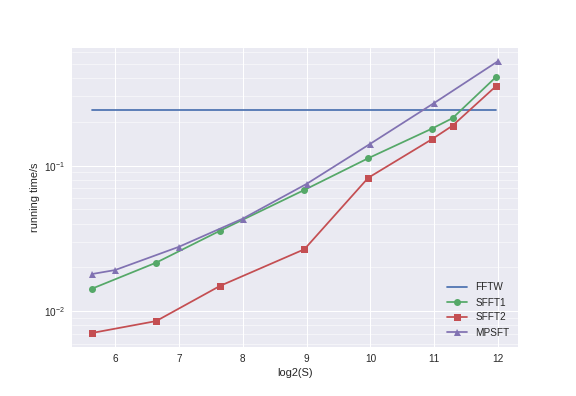
\includegraphics[scale=0.6]{./graph/runtime_vary_k}
\caption{Loglog plot of running time versus sparsity $S$. Runtime of MPSFT is roughly linear with $S$. \label{fig:runtime_vary_k}}
\end{figure}

\subsection{Experiment: Fix $N$, vary $S$}
Use the same parameters as the last experiment. The only difference is that we fix $S=50$ and increase $N$. The results are plotted in Figure \ref{fig:runtime_vary_n}.

We see that FFTW runtime has roughly a linear relationship with $N$ as expected. MPSFT runtime grows very slowly with $N$. It is faster than sFFT1 when $N \gtrsim 2^{23}$, and faster than sFFT2 when $N \gtrsim 2^{25}$.

\begin{figure}
\centering
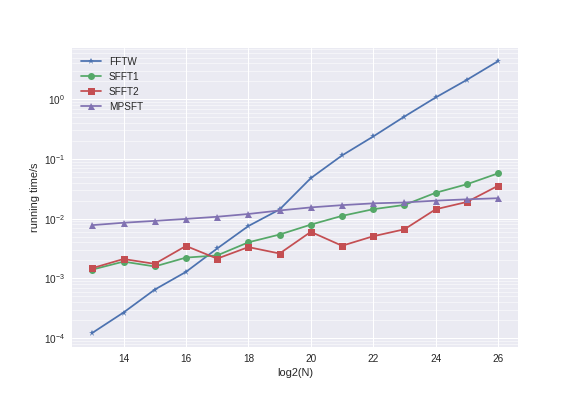
\includegraphics[scale=0.6]{./graph/runtime_vary_n}
\caption{Loglog plot of running time versus $N$. Runtime of MPSFT is roughly independent of $N$. \label{fig:runtime_vary_n}}
\end{figure}

\subsection{Experiment: Vary amount of noise}

Use the same parameters as the previous section except that the minimum number of bins is set to $101$.

Fix $S=1024$ and vary $\sigma$. Define the $L_1$ error or mean absolute error as $\frac{1}{N}\sum_k |\hat{x}_k - \hat{x}^{\text{est}}_k|$. We plot the mean $L_1$ error versus $\sigma$ on a log-log scale in Figure \ref{fig:noise}. Observe that this $L_1$ error scales linearly with $\sigma$. This shows that MPSFT is robust to noise.

\begin{figure}
\centering
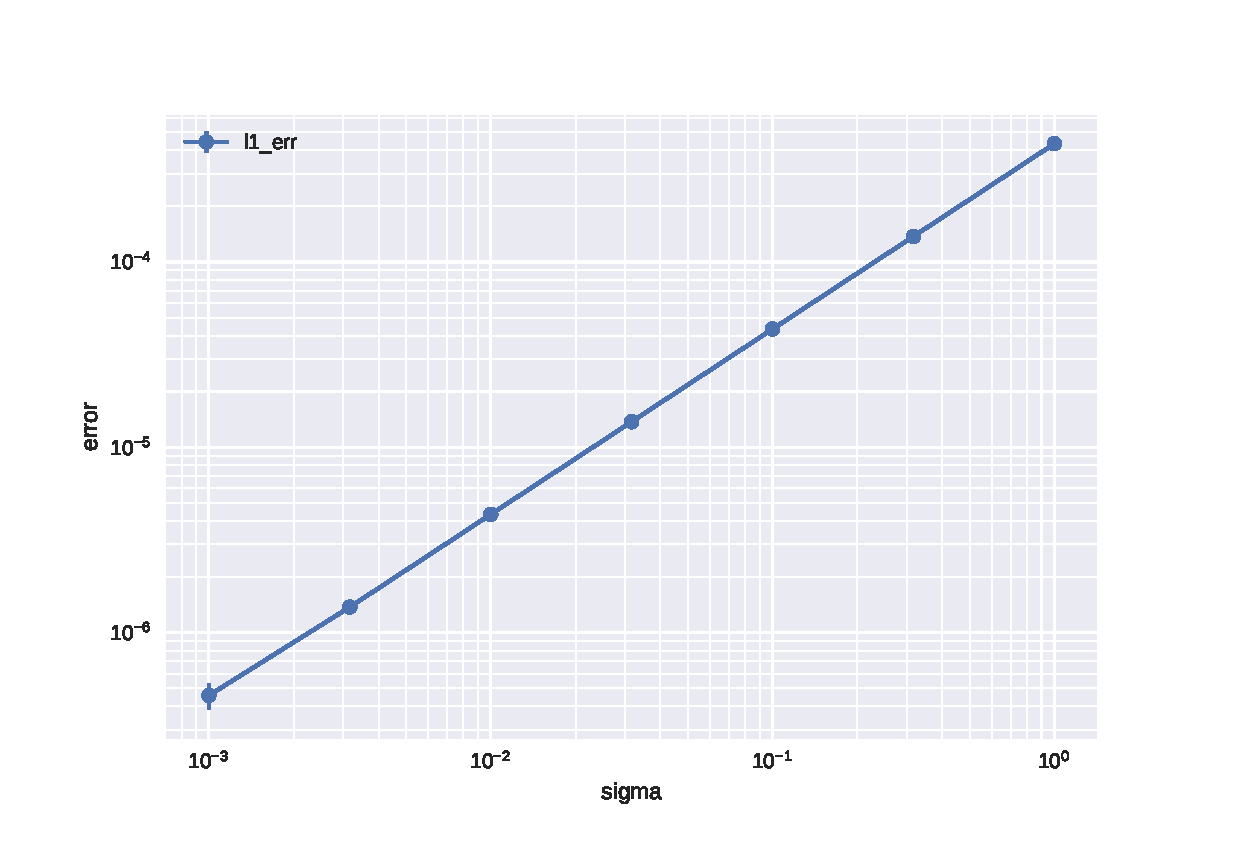
\includegraphics[scale=0.6]{./graph/noise}
\caption{Loglog plot of mean $L_1$ error versus $\sigma$. The mean $L_1$ error grows roughly linearly with $\sigma$. Errorbars are included and very small. \label{fig:noise}}
\end{figure}

\subsection{Benchmarking binning}
From code profiling, we observe that binning dominates the runtime of MPSFT. Hence, as we make various optimizations, we record the improvement in binning speed.

\begin{center}
\begin{tabular}{|c|c|c|}
\hline
Version & Running time/ns & Remarks \\
\hline
BinInTimeV0 & 51313717 & Reference implementation \\
BinInTimeV1 & 33825153 & Exploit symmetry \\
BinInTimeV2 & 15464899 & Chebyshev approximation \\
BinInTimeV3 & 15498434 & Boost.SIMD \\
BinInTimeV4 & 13177513 & Work with double instead of complex arrays \\
BinInFreqV0 & 189515 & Reference implementation \\
BinInFreqV1 & 91742 & Exploit symmetry\\
\hline
\end{tabular}
\end{center}

After applying the results in Section \ref{sec:symmetry}, \texttt{BinInTime} and \texttt{BinInFreq} achieve a 1.5X and 2.1X speedup respectively. After applying vectorization, \texttt{BinInTime} achieves another 2.2X speedup. Finally, by working with double arrays instead of complex arrays, \texttt{BinInTime} receives a modest 1.2X speedup.

\bibliographystyle{abbrv}
\bibliography{references}

\end{document}